\chapter{Class diagram}
\section{Common Layer}
The class diagram shown in figure \ref{fig:commonoverview} gives an overview of all the classes (but doesn't show all the relations!). This overview is to clarify that the \emph{FlowNetworkEntity} have a \texttt{"has-a"} relationship with the components (\emph{MergerEntity, PumpEntity...}).

In figure \ref{fig:classcomponents} the class diagram gives a more detailed view of the components and in more detail how the pipes are connected. Very noticeable are the interfaces \emph{IFlowOutput} and \emph{IFlowInput}. Since a component can have more than 1 input/output an array is used, whereby the pipe also needs to understand to which output it is connected hence the pipe also has the index pipe.

\section{Presentation Layer}
The presentation layer as shown in figure \ref{fig:presentationoverall} has left out a lot of logic, e.g. click events ands such since it is redundant to the reader. View-models are used to edit the properties of selected components. The \emph{ViewModelBase} is an abstract class for all the view-models, using data-binding the data is shown on the screen. If the end-user edits a property an event will be triggered back. This isn't possible with the graphics since it works best with text and not with graphics manipulation. When data is changed it will be triggered to the business layer.

\section{Business Layer}
The class diagram of the Business Layer can be seen in figure \ref{fig:businesslayer} contains all the business logic. This layer has no classes derived from the components from the common layer (e.g. there is no PumpModel). That is since the business layer manipulates the objects from the common layer. Like when the flow network needs to be updated it will use the implementation of \emph{IFlowCalculator}. 

\section{Data Access layer}
Figure \ref{fig:dataaccess} shows the class diagram of the Data Access layer, the Data Access Layer is small and it could be considered to move this to the business layer. When you open a file you get a dumb model back (objects from common) because otherwise the system is failing to follow Separation of Concerns in SOLID principals.

\begin{figure}[h!]
	\centering
	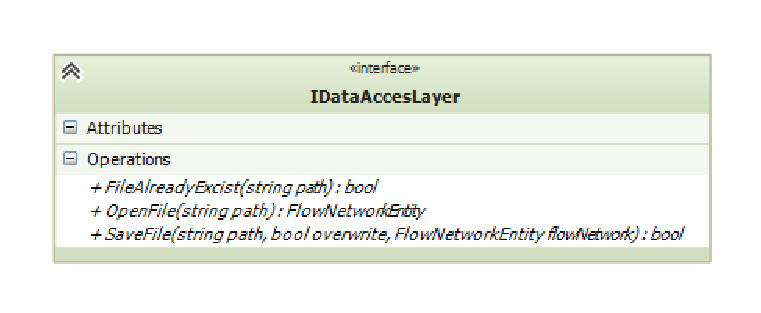
\includegraphics{figures/ClassDataAccess.pdf}
	\caption{Class Diagram Data Access Layer}
	\label{fig:dataaccess}
\end{figure}

\begin{sidewaysfigure}[h!]
	\centering
	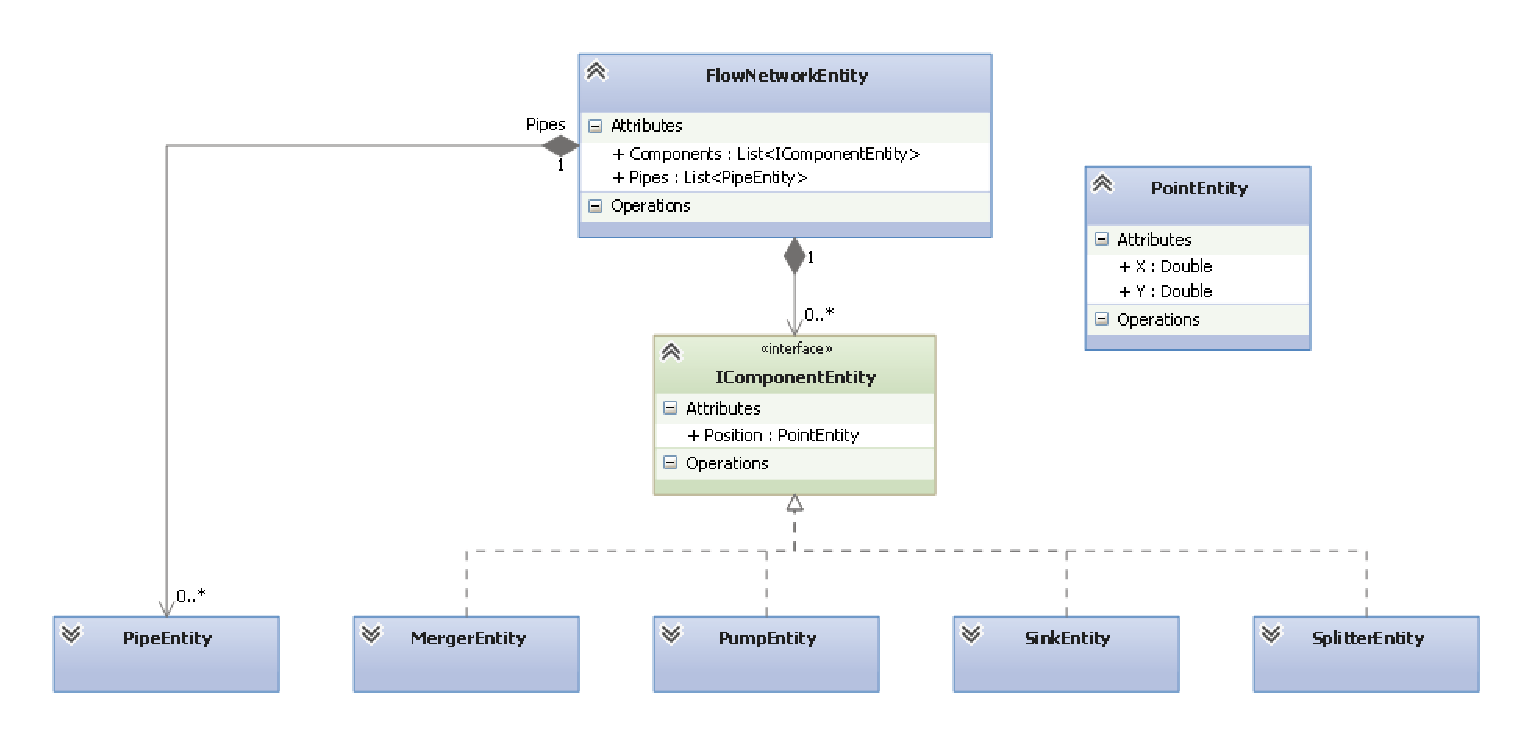
\includegraphics[width=\textwidth]{figures/ClassCommonOverall.pdf}
	\caption{Class Diagram Common overview}
	\label{fig:commonoverview}
\end{sidewaysfigure}

\begin{sidewaysfigure}[h!]
	\centering
	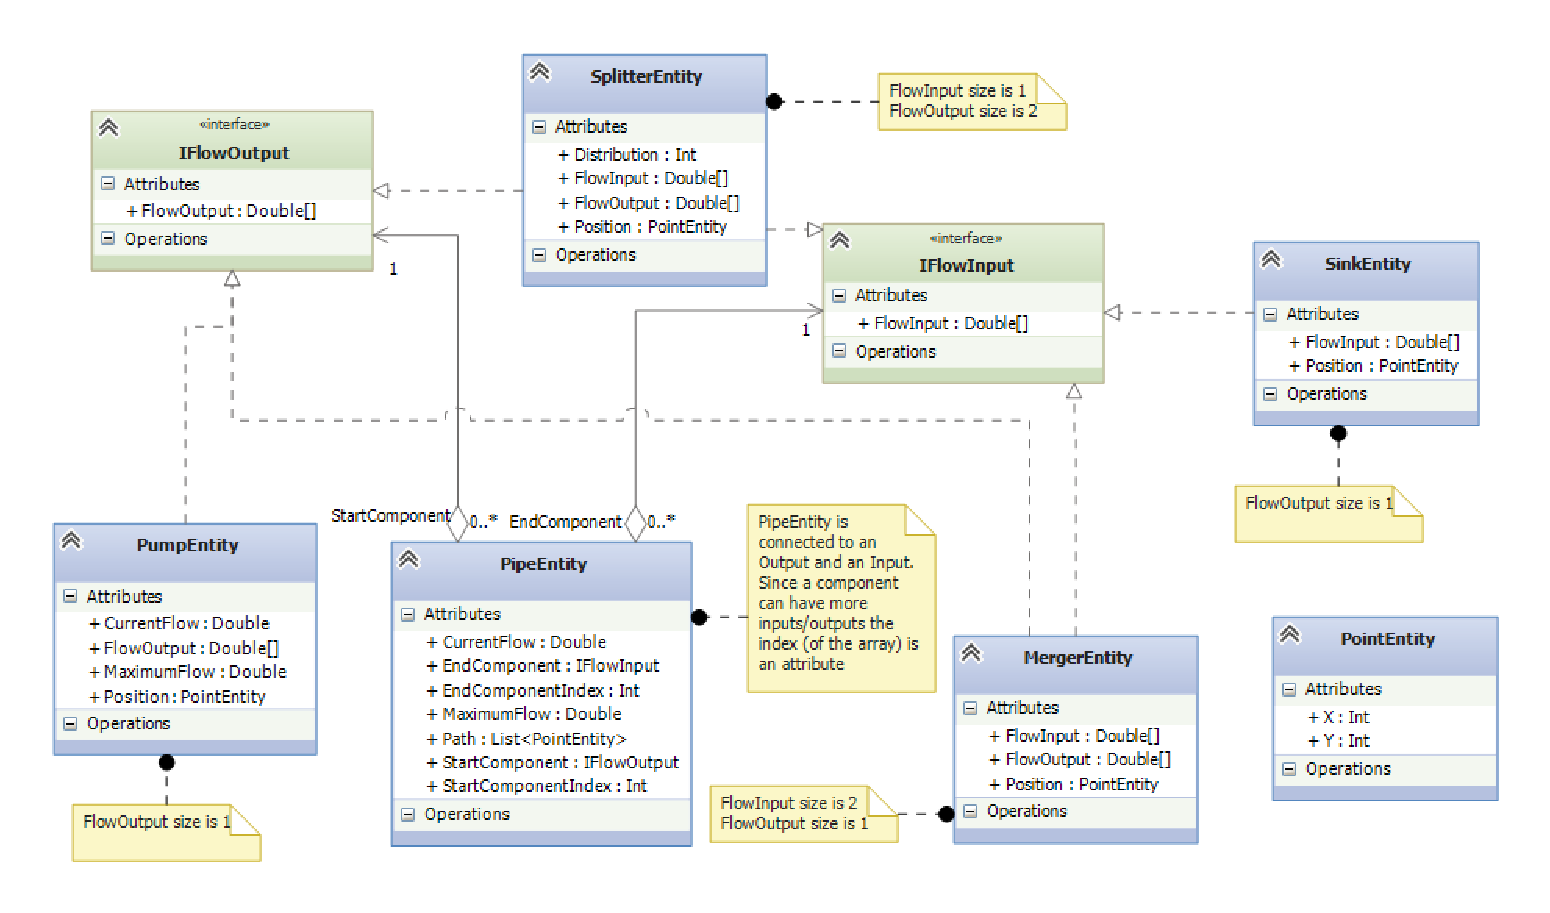
\includegraphics[width=\textwidth]{figures/ClassCommonComponents.pdf}
	\caption{Class Diagram Common Components}
	\label{fig:classcomponents}
\end{sidewaysfigure}

\begin{sidewaysfigure}[h!]
	\centering
	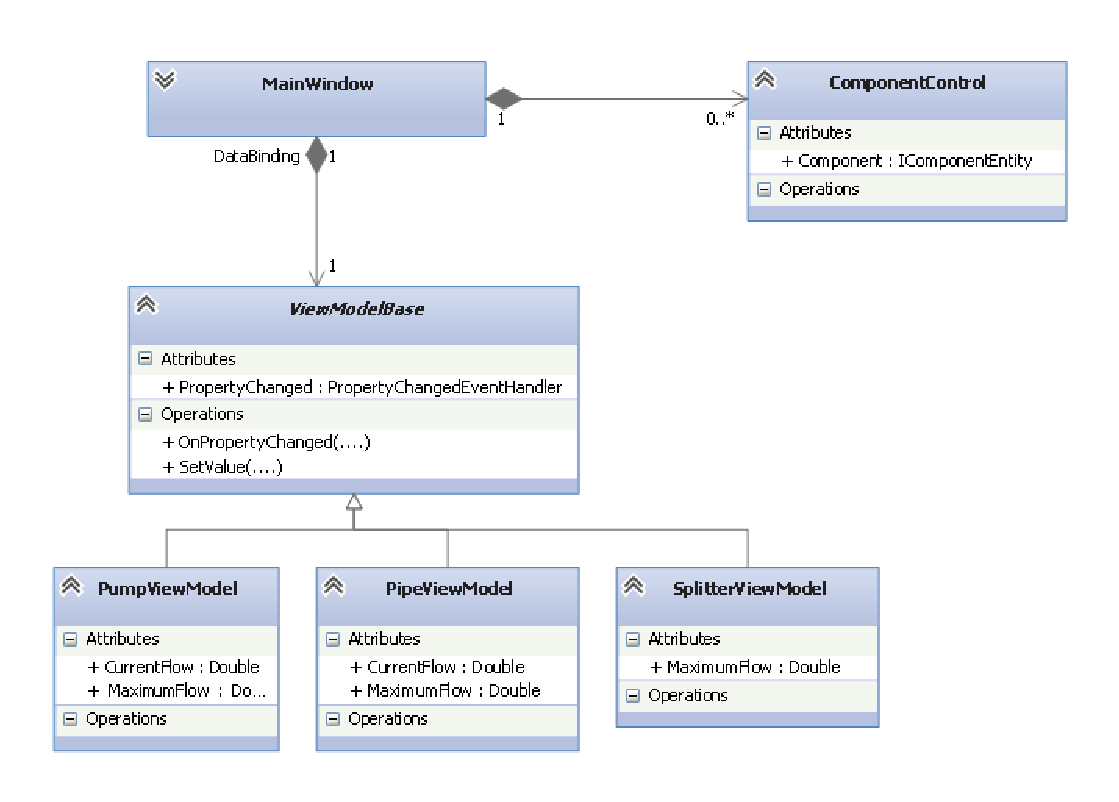
\includegraphics[width=\textwidth]{figures/PresentationOverall.pdf}
	\caption{Class Diagram Presentation Layer}
	\label{fig:presentationoverall}
\end{sidewaysfigure}

\begin{sidewaysfigure}[h!]
	\centering
	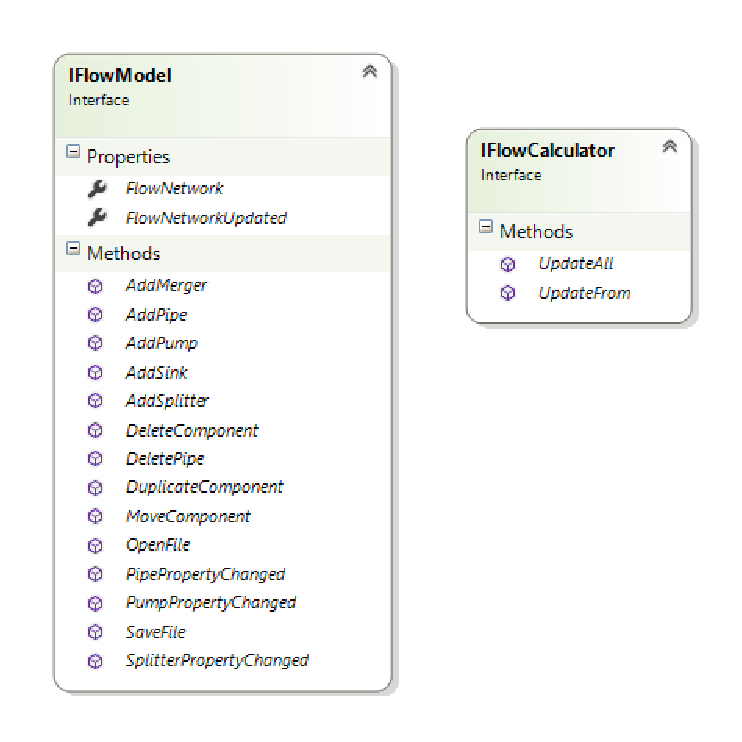
\includegraphics[width=\textwidth]{figures/BusinessOverall.pdf}
	\caption{Class Diagram Business Layer}
	\label{fig:businesslayer}
\end{sidewaysfigure}